\section{Background}
The number of parcels of water and sediment used for the weighted random walks influences the sensitivity of the model to extreme events \cite{Liang2015, Liang2015a}.
Therefore it is important to understand the relationship between the number of parcels used for a given model run and the runtime required.
This type of knowledge can help guide numerical experiment design. 

\section{Model Runs}
A set of 36 model runs, each with a different number of water parcels (\textit{Np\_{}water}) and a different number of sediment parcels (\textit{Np\_{}sed}) were conducted on a mini-domain.
The YAML below provides information about the domain and parameters used.\\

\noindent \texttt{YAML} configuration file: \vspace{-6pt}
\begin{boxedverbatim}
timesteps: 500
Length: 3000.0
Width: 5000.0
seed: 0
dx: 50.0
L0_meters: 50.0
N0_meters: 250.0
h0: 5.0
SLR: 36e-10  # small background SLR
save_dt: 250000

matrix:
  Np_sed:
    - 500
    - 1000
    - 1500
    - 2000
    - 2500
    - 3000
    
  Np_water:
    - 500
    - 1000
    - 1500
    - 2000
    - 2500
    - 3000
\end{boxedverbatim}

\section{Results}
The relationship between runtime, the number of water parcels, and the number of sediment parcels is plotted in 3-D space to inspect impact of the parcels on the time it takes for the model to run (Figure \ref{fig:np_v_runtime}).

\begin{sidewaysfigure}[!htbp]
	\makebox[\textwidth][c]{
	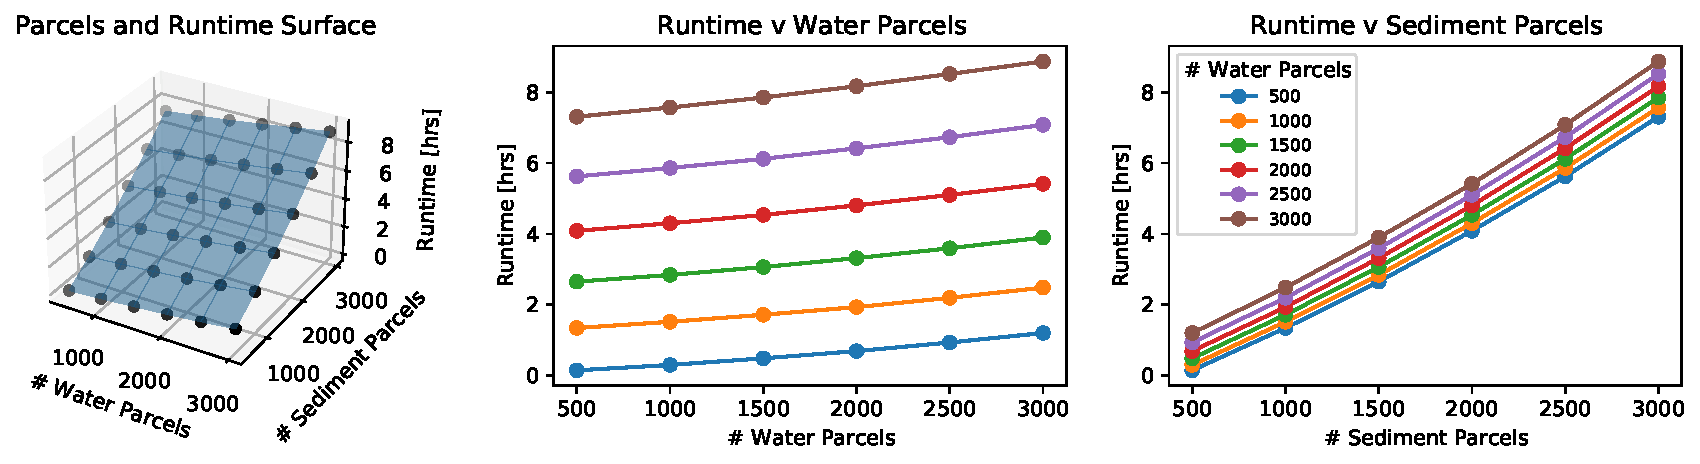
\includegraphics[width=\textwidth]{NumParcelsRuntime/figs/parcels_v_runtime.pdf}
	}	
	\caption{Results from the 36 runs. \textit{Left:} 3-D surface relating the number of water and sediment parcels to runtime. \textit{Center:} 2-D plot of runtime versus the number of water parcels, color indicates number of sediment parcels. \textit{Right:} Run time as a function of the number of sediment parcels, color indicates number of water parcels.}
	\label{fig:np_v_runtime}
\end{sidewaysfigure}

\section{Conclusions}
Water routing is computationally much cheaper than sediment routing as the cohort of parcels is routed in parallel.
This makes the increase in runtime for a greater number of water parcels much less dramatic than the increase in runtime when additional sediment parcels are used.
Increasing the number of sediment parcels can drastically raise the runtime required as these parcels are routed in serial, as each one modifies the topography as it moves through the domain.

\clearpage
\bibliographystyle{plainnat}
\bibliography{bib/bib}